% -------------------------------------------------------- %
% Report for Isaac D. Scherson
% by: Dario Bahena Tapia
% by: Ricardo Zavaleta Vazquez
% by: Isai Barajas Cicourel


% -------------------------------------------------------- %
% Document Start
\documentclass[letter,12pt]{report}


% -------------------------------------------------------- %
% Packages
\usepackage{algorithmic}
\usepackage{amssymb}
\usepackage{amsfonts}
\usepackage{color}
\usepackage{xcolor}
\usepackage{graphicx}
\usepackage{caption}
\usepackage{listings}
\usepackage{listings,multicol}
\usepackage{graphicx}
\graphicspath{ {images/} }


% -------------------------------------------------------- %
% Document
\begin{document}


% --------------------------- %
% Title Page Start
% --------------------------- %
\begin{titlepage}
\begin{center}

~\\[4 cm]


\includegraphics[width=15 cm]{Oracle_Logo.pdf}

~\\[0.5 cm]

% Document Information
{\LARGE Multiprocessor Programming Course} \\[0.2 cm]

% Names
{Dario Bahena Tapia - Ricardo Zavaleta Vazquez - Isai Barajas Cicourel}

% Date
{\small October 2015}

\end{center}
\end{titlepage}
% --------------------------- %
% Title Page End
% --------------------------- %


% --------------------------- %
% Mutual Start
% --------------------------- %
\chapter{Mutual Exclusion}
\section{Problem Definition}
../../zava/Multiprocessor//Peterson.tex
% --------------------------- %
% Bakery Start
% --------------------------- %
\section{\textbf{Bakery Test}}
%%%%%%%%%%%%%%%%%%%%%%%%%%%%%%%%%%
\subsection{Particular Case}
\par
In this experiment, we are dealing with the problem of mutual exclusion with a
number of participants $>2$.
\par
We have already seen that Peterson Algorithm works for two threads. It garantees
mutual exclusion and is starvation free. Therefore, the algorithm is deadlock
free. Now let us focus in an algorithm that can be used to coordinate more
threads.
\par
%%%%%%%%%%%%%%%%%%%%%%%%%%%%%%%%%%
\subsection{Solution}
\par
The algorithm that we will play with is called \textit{Bakery}. Its name comes from the
fact that it is similar to the protocol used in bakeries where one enters the
store and picks a number that indicates the order in which each client will be
attended. 
\par
In the algorithm, the fact of entering the store is done by setting a flag.
After that, the thread calculates the next number in the machine. 
\par
The algorithm then chooses the next number to be attended. When that happens,
the thread is allowed to enter the critical section.
\par
One thing that we ougth to mention is that threads can have the same number
assigned. If that is the case, the next in the line is decided using a
lexicographical ordering of the threads ids.
\par
Here we show the interesting methods used in this algorithm:
\par
\hfill
\begin{lstlisting}[style=numbers]
  public void lock() {
    int me = ThreadID.get();
    flag[me]  = true;
    int max = Label.max(label);
    label[me] = new Label(max + 1);
    while (conflict(me)) {};  // spin
  }

  public void unlock() {
    flag[ThreadID.get()] = false;
  }
  
  private boolean conflict(int me) {
    for (int i = 0; i < label.length; i++) {
      if (i != me && flag[i] && label[me].compareTo(label[i]) < 0) {
        return true;
      }
    }
    return false;
  }

  static class Label implements Comparable<Label> {
    int counter;
    int id;
    Label() {
      counter = 0;
      id = ThreadID.get();
    }
    Label(int c) {
      counter = c;
      id = ThreadID.get();
    }
    static int max(Label[] labels) {
      int c = 0;
      for (Label label : labels) {
        c = Math.max(c, label.counter);
      }
      return c;
    }
    
    public int compareTo(Bakery.Label other) {
      if (this.counter < other.counter
          || (this.counter == other.counter && this.id < other.id)) {
        return -1;
      } else if (this.counter > other.counter) {
        return 1;
      } else {
        return 0;
      }
    }
  }
\end{lstlisting}
\hfill
\par
In the \textit{lock()} method, we observe that the thread signals its intention
of accessing the critical section by setting its flag to true. After that, the
thread picks its number and then it sits and waits for its turn. The thread has
to wait if another thread which announced its intention to use the resource has
a smaller label. 
\par
%%%%%%%%%%%%%%%%%%%%%%%%%%%%%%%%%%
\subsection{Experiment Description}
\par
Now let us explain how the experiments work. In this case we have 8 threads
increasing a counter from 0 to 1024. Each thread will increase the counter 128
times. At the end, the counter must remain in 1024. If that is not the case,
then there is a problem with the mutual exclusion algorithm.
\par
%%%%%%%%%%%%%%%%%%%%%%%%%%%%%%%%%%
\subsection{Sample Results}
\par
In this exercise we observed that in the machine that we have been using, the
test for the Bakery algorithm fails consistently with the following error:
\par
\begin{verbatim}
.F
Time: 0.019
There was 1 failure:
1) testParallel(mutex.BakeryTest)junit.framework.AssertionFailedError:
expected:<1019> but was:<1024>
        at mutex.BakeryTest.testParallel(BakeryTest.java:47)
        at sun.reflect.NativeMethodAccessorImpl.invoke0(Native Method)
        at
sun.reflect.NativeMethodAccessorImpl.invoke(NativeMethodAccessorImpl.java:57)
        at
sun.reflect.DelegatingMethodAccessorImpl.invoke(DelegatingMethodAccessorImpl.java:43)

FAILURES!!!
Tests run: 1,  Failures: 1,  Errors: 0
\end{verbatim}
\par
%%%%%%%%%%%%%%%%%%%%%%%%%%%%%%%%%%
\subsection{Interpretation}
\par
Let us elaborate on the meaning of the error that we got. The assertion failure
says that at the end of the algorithm, our counter didn't reach the expected
1024. This problem might indicate that our counter wasn't actually being
protected by the lock because it looks like multiple threads found the counter
with a value of $i$ and increased it to $i+1$. This is wrong.
\par
After investigating the problem in more detail, we found out that the problem in
this code has to do with the way the \textit{label} array is accessed and
modified. For example, in the lock method, multiple threads can reach the point
where the max is calculated and hence these mutiple threads can take the same
turn. The algorithm takes care of this problem by introducing a lexicographical
ordering in the comparison: if two threads have the same number, the decision is
made based on the $threadID$.
\par
Also, as explained in the textbook, we cannot be sure that we have a correct
memory consistency: it is possible that the processor modified the order in
which operations in the \textit{lock()} method are executed. It is also possible
that the processor decided to execute an instruction before another.
\par
%%%%%%%%%%%%%%%%%%%%%%%%%%%%%%%%%%
\subsection{Proposed solution}
\par
The following fragment of code shows one possible way of fixing the code:
\par
\hfill
\begin{lstlisting}[style=numbers]
  public void lock() {
    int me = ThreadID.get();
    flag[me]  = true;
    synchronized (label){
      int max = Label.max(label);
      label[me] = new Label(max + 1);
      while (conflict(me)) {};  // spin
    }
  }
\end{lstlisting}
\hfill
Note that this solution is not quite satisfactory as we are basically using a
Java mechanism to ensure synchronized access in an algorithm that promises to
provide synchronized access.
\par
In any case, let us show the output of the program after this fix:
\begin{verbatim}
.
Time: 0.015

OK (1 test)
\end{verbatim}
\hfill
\par
After the fix the results in the proposed system were all OK. In all cases, the
threads were able to cooperate to increase the counter to 1024.
\par
One thing that is worth mentioning is that unlike the Peterson Algorithm, for
example, the Bakery algorithm is able to coordinate multiple threads (at least
in theory). This fact was shown in the test case were 8 threads were coordinated
to increase the counter.
%%%%%%%%%%%%%%%%%%%%%%%%%%%%%%%%%%
% --------------------------- %
% Bakery End
% --------------------------- %

% --------------------------- %
% Mutual End
% --------------------------- %

\chapter{Foundations of Shared Memory}
\section{\textbf{Safe Boolean MRSW Register}}
% ------------------------------------------------------------------------------------ %
\subsection{Particular Case}
\par
In class we saw the difference between Safe, Regular and Atomic Registers. In
this excersice we are experimenting with a Safe Boolean Register. In particular,
we are trying a register that allows one single writer whose writen value can be
examined by multiple readers. We need to remember that Safe registers are those
that :
\begin{itemize}
\item If a read does not overlap with a write, then the read returns the last
written value
\item If a read overlaps with a write, then the read can return any value in the
domain of the register's values
\end{itemize}
% ------------------------------------------------------------------------------------ %
\subsection{Solution}
\par
One way to achive this behaviour is using a SRSW Safe register. The code that is
provided with the book does this by having a boolean SRSW register per thread,
in other words, it is an array of boolean values. When doing a write, the writer
iterates over this array and writes the new value. The readers simply access its
assigned slot in the array (based on the thread id) and return the stored value. 
% ------------------------------------------------------------------------------------ %
\subsection{Experiment Description}
\par
This program provides two test cases. The first one is a sequential test and the
second one is a parallel test. The former simply calls a write and then a read
from the same thread. This is not rocket science. The reader must retrieve what
the writer wrote.
\par
The second test case is slightly more interesting. The writer writes first one
value and then another one. After that, 8 reader threads are started and they
read the last written value. According to the rules of a safe register, al
threads must read the same value because the reads and the writes did not
overlap.
\par
These are the details of the system we used to run the experiments:
\begin{itemize}
\item Processor: Intel Core i5 @2.5 GHz. 2 Cores.
\item L2 Cache per Core: 256 KB
\item L3 Cache: 3 MB
\item System Memory: 16 GB
\end{itemize}
% ------------------------------------------------------------------------------------ %
\subsection{Sample Results}
We found out that the tests failed ocassionally. The manifestation of such
failures were two:
\begin{enumerate}
\item The jUnit framework reports a failure in one of the tests as shown in
figure \ref{fig:SafeBooleanMRSW00}
\item The jUnit doesn't report a failure, however the test output shows an
\textit{Out of Bounds exception}. This is shown in figure
\ref{fig:SafeBooleanMRSW01}
\end{enumerate}
\par
\begin{figure}[h]
  \centering
  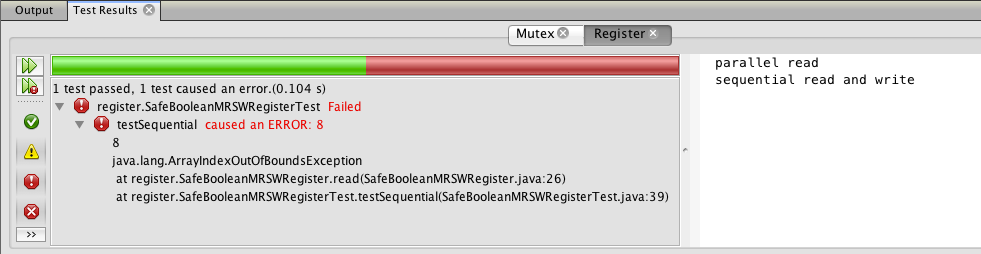
\includegraphics[width=13cm]{SafeBooleanMRSW00.png}
  \caption{First type of failure}
  \label{fig:SafeBooleanMRSW00}
\end{figure}
\par
\begin{figure}[h]
  \centering
  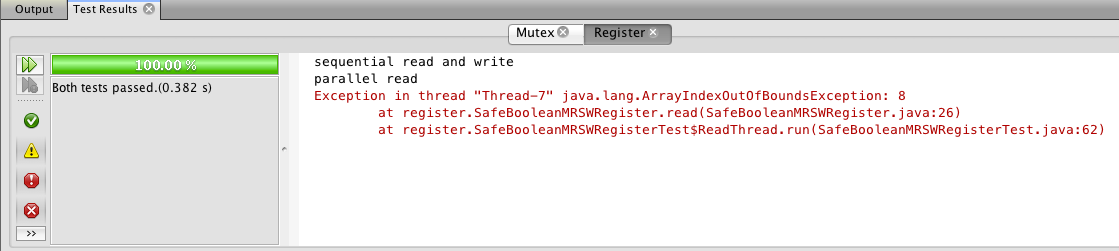
\includegraphics[width=13cm]{SafeBooleanMRSW01.png}
  \caption{Second type of failure}
  \label{fig:SafeBooleanMRSW01}
\end{figure}
\par
So, the way to fix this problem was to make sure that in each test case
the threads ids are reset calling the static method $ThreadID.reset()$. With
this hack, the tests passed (See figure \ref{fig:SafeBooleanMRSW02}).
\par
\begin{figure}[h]
  \centering
  \includegraphics[width=13cm]{SafeBooleanMRSW02.png}
  \caption{Output after fix}
  \label{fig:SafeBooleanMRSW02}
\end{figure}
\par
\begin{figure}[h]
  \centering
  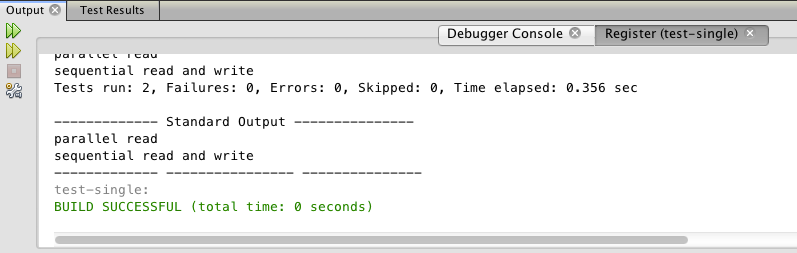
\includegraphics[width=13cm]{SafeBooleanMRSW03.png}
  \caption{Output after fix of threadIds}
  \label{fig:SafeBooleanMRSW03}
\end{figure}
\par
% ------------------------------------------------------------------------------------ %
\subsection{Interpretation}
\par
In this experiment we saw a way of implementing Safe Multi-Reader Single-Writer
registers. These registers were able of storing boolean values.
\par
Unfortunately, none of the test cases excersice the case where we have
concurrent writes and reads. Hence, this experiment only excersiced one of the
two rules of a safe register.
% ------------------------------------------------------------------------------------ %

\section{\textbf{Atomic MRSW Register}}
% -------------------------------------------------------------------------------- %
\subsection{Particular Case}
\par
The characteristics of this type of register are:
\begin{itemize}
\item It should never happen that $R^{i} \rightarrow W^{i}$
\item It should never happen that for any ${j}$, ${W^{i} \rightarrow W^{j} \rightarrow R^{j}}$
\item If ${R^{i} \rightarrow R^{j}}$ then ${i \leq j}$
\end{itemize}
The book proposes to do this by using multiple SRSW registers.
% -------------------------------------------------------------------------------- %
\subsection{Solution}
The algorithm then requires a 2 dimensional table. When a writer decides to
update the register, it has to update the values in cells $A[i][i]$, where $i$
is the thread id. Apart from writing the value, it has to also update the cell
with a timestamp. 
\par
In the other hand, when a reader wants to read from the register, it checks the
timestamp of the cell $A[i][i]$. After that, it has to check other cells in the
same column (ie, cells $A[x][i]$) to see if there has been an update in between.
That is done by comparing the timestamps. If there is a newer timestamp, the
reader has then to update all cells in its row (ie $A[i][x]$). This is the way
to indicate subsequent readers which version of the value has the previous
reader retrieved.
\par
It is easy to see that the first property is satisfied because there is no way
to read a future value. In order to read a value, this value has to be written
before.
\par
The second property is also satisfied because when a reader reads the value, it
reads the one with the most recent timestamp by scaning the timestamps in its
corresponding column. This reader also helps subsequent readers by updating all
cells in its row. Forcing property 3 to be satisfied as well.
\par
% -------------------------------------------------------------------------------- %
\subsection{Experiment Description}
\par 
The two test cases presented demonstrates the same as previous examples so we
will not describe the experiment further. 
\par
These are the details of the system we used to run the experiments:
\begin{itemize}
\item Processor: Intel Core i5 @2.5 GHz. 2 Cores.
\item L2 Cache per Core: 256 KB
\item L3 Cache: 3 MB
\item System Memory: 16 GB
\end{itemize}
% -------------------------------------------------------------------------------- %
\subsection{Sample Results}
As in previous examples, we identified that the test fails from time to time.
Figure \ref{fig:AtomicMRSW00} shows the output when the failure is seen.
\par
\par
\begin{figure}[h]
  \centering
  \includegraphics[width=13cm]{AtomicMRSW00.png}
  \caption{First type of failure}
  \label{fig:AtomicMRSW00}
\end{figure}
\par
Again, the fix for these failures was to reset the thread ids.
\par
\begin{figure}[h]
  \centering
  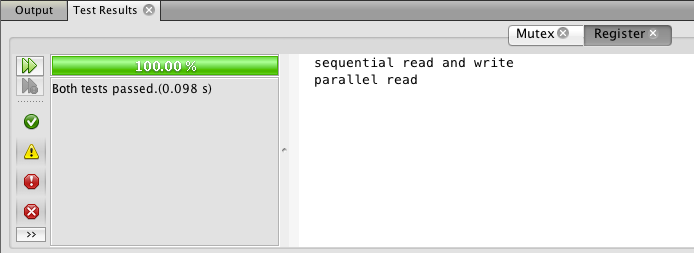
\includegraphics[width=13cm]{AtomicMRSW01.png}
  \caption{Output after fix}
  \label{fig:AtomicMRSW01}
\end{figure}
\par
\begin{figure}[h]
  \centering
  \includegraphics[width=13cm]{AtomicMRSW02.png}
  \caption{Output after fix of threadIds}
  \label{fig:AtomicMRSW03}
\end{figure}
\par
% -------------------------------------------------------------------------------- %
\subsection{Interpretation}
\par
In this experiment we observed a way of implementing MRSW registers. We saw
that, at least in the processor we used, the algorithm seems to work correctly.
\par
It would have been great, though, to also have test cases that demonstrate that this
particular register satisfies property 3 which is the one that makes it
different from the Safe version.
% -------------------------------------------------------------------------------- %

\section{\textbf{Wait-Free Snapshots}}
% ---------------------------------------------------------------------------- %
\subsection{Particular Case}
\par
In this experiment we are dealing with the problem of creating an algorithm to
create a Snapshot of a set of Register in such a way that the algorithm
guarantees a Wait-Free operation.
\par
% ---------------------------------------------------------------------------- %
\subsection{Solution}
\par
The purpose of a Wait-Free snapshot is to overcome the problems of the Simple
snapshot presented before. Let us remember that such snapshot executes successive
collect() operations. Once it achieves a \textit{clean double collect}, it
returns the snapshot. Otherwise, it uses the following idea:
\par
When a double collect fails, it is because a update interfered. That means that
the updater could take a snapshot right before its update and other threads
could use it as their snapshot too. 
\par
Since this algorithm is a bit more complex, let us explain in more detail how
the implementation works.
\par
\hfill
\begin{lstlisting}[style=numbers]
  public WFSnapshot(int capacity, T init) {
    a_table = (StampedSnap<T>[]) new StampedSnap[capacity];
    for (int i = 0; i < a_table.length; i++) {
      a_table[i] = new StampedSnap<T>(init);
    }   
  }
\end{lstlisting}
\hfill
\par
Firstly, the algorithm uses an array to store the information.
The size of the array is, in this case, $n$, where $n$ is the number of
threads. The way in which this array is constructed is as an array of
\textit{StampedSnap}s. A StampedSnap is internally an array whose elements are
of type \textit{T}. A StampedSnap is a subclass of StampedValue which has 3
fields:
\par
\begin{itemize}
\item \textit{stamp}, which is a counter
\item \textit{owner}, which contains the thread id
\item \textit{value}, the actual value in the register
\end{itemize}
\par
Now let us look at an auxiliar operation which is \textit{collect()}. This
operation returns a copy of the array. Observe that the method creates a new
array of StampedSnap values and then iterates the existing array to copy each element.
\par
\hfill
\begin{lstlisting}[style=numbers]
  private StampedSnap<T>[] collect() {
    StampedSnap<T>[] copy = (StampedSnap<T>[]) new StampedSnap[a_table.length];
    for (int j = 0; j < a_table.length; j++)
      copy[j] = a_table[j];
    return copy;
  }
\end{lstlisting}
\hfill
\par
The next method to understand is \textit{scan()}. The method first creates a
backup or an old copy of the array. Then it takes a second collect. It then
compares both copies. If both copies are equal, then it means that we have a
double clean collect. And the result of the scan operation is any of the copies
just as in the Sequential Snapshot case.
\par
On the other hand, if the copies are different, then there are two cases. For
this, we have a counter that indicates how many times, the copies have been
compared and found different. If it is the first time, then we take another
collect. If in the second collect, the copies are equal, then we fall in the
case described in the previous paragraph. If the copies are different again,
then it means that we can take the old copy as a result of the scan. 
\par
The justification of this is that if a thread A sees a thread B move twice while
it is performing repeated collects, then B executed a complete \textit{update()}
call within the interval of A's scan, and so it is correct for A to use B's
snapshot.
\par
\hfill
\begin{lstlisting}[style=numbers]
  public T[] scan() {
    StampedSnap<T>[] oldCopy;
    StampedSnap<T>[] newCopy;
    boolean[] moved = new boolean[a_table.length];
    oldCopy = collect();
    collect: while (true) {
      newCopy = collect();
      for (int j = 0; j < a_table.length; j++) {
        // did any thread move?
        if (oldCopy[j].stamp != newCopy[j].stamp) {
          if (moved[j]) {       // second move
            return oldCopy[j].snap;
          } else {
            moved[j] = true;
            oldCopy = newCopy;
            continue collect;
          }   
        }   
      }   
      // clean collect
      T[] result = (T[]) new Object[a_table.length];
      for (int j = 0; j < a_table.length; j++)
        result[j] = newCopy[j].value;
      return result;
    }   
  }
\end{lstlisting}
\hfill
\par
Finally, we have the \textit{update()} operation which simply updates the
register with the new stamp.
\par
\hfill
\begin{lstlisting}[style=numbers]
  public void update(T value) {
    int me = ThreadID.get();
    T[] snap = this.scan();
    StampedSnap<T> oldValue = a_table[me];
    StampedSnap<T> newValue =
      new StampedSnap<T>(oldValue.stamp+1, value, snap);
    a_table[me] = newValue;
  }
\end{lstlisting}
\hfill
% ---------------------------------------------------------------------------- %
\subsection{Experiment Description}
\par
In this experiment, the test looks a bit different. Let us explain how. In this
case we have two experiments:
\par
\begin{enumerate}
\item testSequential. We spawn a new thread that updates the register with a
value of \textit{FIRST} and right after that, it scans the value of the
register. The expected result is that this read retrieves the value of
\textit{FIRST}
\item testParallel. We spawn \textit{THREADS} number of threads (in our case it
is $2$). Each of them will first update its register with a value of
\textit{FIRST} and then with a value of \textit{SECOND}. Each thread then
updates a position in a matrix of size \textit{THREADS}$x$\textit{THREADS} with
the result of doing a $scan()$ operation. At the end we compare consecutive rows
in the matrix. The comparison is done entry by entry and we should see that for
some entries the first entry is greater and for some others it is smaller than
the second. What we must see is that all entries are equal and we allow the
first to sometimes be either greater or smaller than the second one.
\end{enumerate}
% ---------------------------------------------------------------------------- %
\subsection{Sample Results}
\par
For this test, we saw that in every try, both test cases passed. Here is the
output:
\par
\begin{verbatim}
[oraadm@gdlaa008 Register]$ junit register.WFSnapshotTest
.sequential
.parallel

Time: 0.003

OK (2 tests)
\end{verbatim}
\par
% ---------------------------------------------------------------------------- %
\subsection{Interpretation}
% ---------------------------------------------------------------------------- %
In this experiment we were able to observe how a Wait-Free Snapshot can be
constructed based on the idea of \textit{clean double collects} and on the idea
of using the updater's collect when the clean double collect method fails.


\chapter{Spin Locks and Contention}
../../zava/Multiprocessor//SpinLocks.tex
../../zava/Multiprocessor//TASLockTest.tex
\section{\textbf{Hierarchical Backoff Lock}}
\subsection{Particular Case}
\par
The specific case we are trying to solve here is that of mutual exclusion with long waiting times on architectures that make use of hierarchical caching. Let us describe more deeply the characteristics of this scenario.
\par
Firstly, it has already been discussed the difference between \textit{spinning} and \textit{backing-off}. The first case consists on doing an active wait in the case where a $lock()$ operation is not successful. On the other hand, a $backoff$ means that the thread
who failed to acquire the lock refraing from retrying for some duration giving competing threads a chance to finish. As mentioned in the book, the idea is to avoid bus traffic caused by threads asking over and over again for the state of the lock.
\par
The term \textit{Hierarchical} comes from the fact that modern cache-coherent architectures organize processors in clusters. These clusters are organized in such a way that intra-cluster communication is faster than inter-cluster communication. So, the idea in this experiment is to find a lock implementation that takes advantage of these access times differences.
\par
\subsection{Solution}
\par
One of the solutions proposed in the book consists on adapting the \textit{test-and-test-and-set} lock that was described in a previous chapter to exploit the characteristics of the cluster. The idea behind this implementation is that backoff times of local threads should be shorter than backoff times of remote threads. 
\par
\subsection{Experiment Description}
\par
To demonstrate that this implementation works, the test that was provided does the following:
\begin{enumerate}
\item Initiate a shared counter with a value of $0$
\item Start $32$ threads
\item Each thread has to increment the counter by one $32$ times
\item At the end, the counter must hold a value of $32*32$
\end{enumerate}
\par
These are the details of the system we used to run the experiments:
\begin{itemize}
\item Processor: Intel Core i5 @2.5 GHz. 2 Cores.
\item L2 Cache per Core: 256 KB
\item L3 Cache: 3 MB
\item System Memory: 16 GB
\end{itemize}
\subsection{Sample Results}
\par
For this test, we saw that in every try, it always passed.
\par
\begin{figure}[h]
  \centering
  \includegraphics[width=5cm]{HBO00.png}
  \caption{Successful execution of the tests for Hierarchichal Back-off test}
  \label{fig:HBO00}
\end{figure}
\par
\begin{figure}[h]
  \centering
  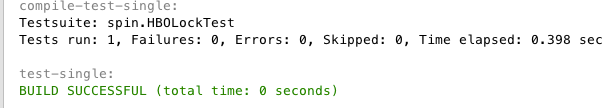
\includegraphics[width=13cm]{HBO01.png}
  \caption{Successful execution of the tests  for Hierarchichal Back-off test}
  \label{fig:HBO01}
\end{figure}
\par
\subsection{Interpretation}
It was shown that the algorithm seems to work and allows synchronization of multiple threads trying to access a shared resource.
\par
One problem however, has to do with the fact that this locking protocol is not fair in the sense that local threads have more chances of acquiring the lock in the next attempt. 
\par
Another thing that we ought to note is that threads spin in the same memory address which causes invalidation of remote cached copies of this value. This problem will be solved yet with another protocol.

\section{\textbf{CLH Queue Lock}}
%%%%%%%%%%%%%%%%%%%%%%%%%%%%%%%%%%
\subsection{Particular Case}
\par
Using queue locks solve two problems that appear in simpler locking protocols.
Firstly, by using a queue, cache-coherence traffic is reduced because each
thread spin on a different memory location; and secondly, by using a queue,
threads can know whether their turn has come by inspecting the status of their
predecesor in the queue.
\par
The particular case that we want to study in this experiment is \textit{How can
we implemente a space efficient Queue Lock?}
\par
%%%%%%%%%%%%%%%%%%%%%%%%%%%%%%%%%%
\subsection{Solution}
\par
One solution for this problem is given by the CLHLock protocol. The algorithm
that implement this protocol need two fields local to the thread: A pointer to
the current node and a pointer to the previous node. The queue is constructed by
having the pointer \textit{previous} pointing to the previous node's
\textit{current} field. This field contains a boolean value which is false when
the thread releases the lock. When this is the case, the next thread is allowed
to acquire the lock. 
\par
%%%%%%%%%%%%%%%%%%%%%%%%%%%%%%%%%%
\subsection{Experiment Description}
\par
To demonstrate that this implementation works, the test that was provided does
the following:
\begin{enumerate}
\item Initiate a shared counter with a value of $0$
\item Start $8$ threads
\item Each thread has to increment the counter by one $1024$ times
\item At the end, the counter must hold a value of $8*1024$
\end{enumerate}
\par
%%%%%%%%%%%%%%%%%%%%%%%%%%%%%%%%%%
\subsection{Sample Results}
\par
In this case, we found that in our 24-cores machine, the test hung. To make it
work, we had to make the \textit{locked} variable in the 
\par
\hfill
\begin{verbatim}
[oraadm@gdlaa008 Spin]$ junit spin.CLHLockTest 
[8] Leaving critical zone
[9] Entering critical zone
[9] Leaving critical zone
[8] Entering critical zone
[8] Leaving critical zone
[9] Entering critical zone
[9] Leaving critical zone
[8] Entering critical zone
[9] Entering critical zone
...
[9] Leaving critical zone
[8] Entering critical zone
[9] Entering critical zone
[8] Leaving critical zone
[8] Entering critical zone
[8] Leaving critical zone

Time: 0.755

OK (1 test)
\end{verbatim}
\hfill
\par
%%%%%%%%%%%%%%%%%%%%%%%%%%%%%%%%%%
\subsection{Interpretation}
It was shown that the algorithm seems to work and allows synchronization of
Multiple threads trying to access a shared variable.
\par
One important thing about this algorith is that threads spin checking for
different memory addresses which avoids invalidation of cached copies. Another
important advantage is that it requieres a limited number of memory and also
provides first-in-first-out fairness. 
\par
The case were this algorithm is not good is when, in a NUMA architecture, the
\textit{previous} pointer points to a remote location. In that case, the
performance of the algorithm degradates.


\chapter{Monitors and Blocking Synchronization}
../../zava/Multiprocessor//CountDownLatch.tex

\chapter{Linked Lists: The Role of Locking}
%\section{\textbf{Coarse List}}
% ---------------------------------------------------------------------------- %
\subsection{Particular Case}
\par
In this experiment we are dealing with the problem of creating an algorithm to
create a Snapshot of a set of Register in such a way that the algorithm
garantees a Wait-Free operation.
\par
% ---------------------------------------------------------------------------- %
\subsection{Solution}
\par
The purpose of a Wait-Free snapshot is to overcome the problems of the Simple snapshot presented before. Let us remember that such snapshot executes sucesive collect() operations. Once it achieves a \textit{clean double collect}, it returns the snapshot. Otherwise, it keeps trying. 
\par
One of the ideas behind the Wait-Free Snapshot is that when a double collect fails, it is because a update interfered. That means that the updater could take a snapshot right before its update and other threads could use it as their snapshot too. 
\par
% ---------------------------------------------------------------------------- %
\subsection{Experiment Description}
\par

\par
These are the details of the system we used to run the experiments:
\begin{itemize}
\item Processor: Intel Core i5 @2.5 GHz. 2 Cores.
\item L2 Cache per Core: 256 KB
\item L3 Cache: 3 MB
\item System Memory: 16 GB
\end{itemize}
% ---------------------------------------------------------------------------- %
\subsection{Sample Results}
\par
For this test, we saw that in every try, both test cases passed.
\par
\begin{figure}[h]
  \centering
  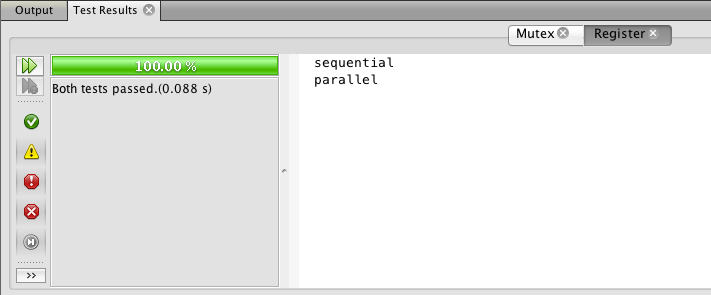
\includegraphics[width=13cm]{WFS00.png}
  \caption{Successful execution of the tests for Wait-Free Snapshot}
  \label{fig:WFS00}
\end{figure}
\par
\begin{figure}[h]
  \centering
  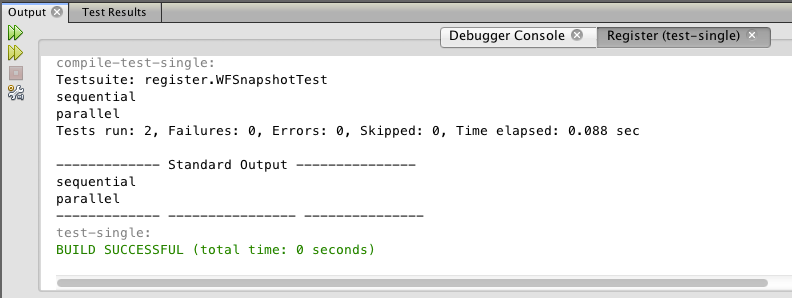
\includegraphics[width=13cm]{WFS01.png}
  \caption{Successful execution of the tests for Wait-Free Snapshot}
  \label{fig:WFS01}
\end{figure}
\par
% ---------------------------------------------------------------------------- %
\subsection{Interpretation}
% ---------------------------------------------------------------------------- %
In this experiment we were able to observe how a Wait-Free Snapshot can be
constructed. 

%\section{\textbf{Lock-Free List}}
% ---------------------------------------------------------------------------- %
\subsection{Particular Case}
\par
We have seen some algorithms for implementing a concurrent list. Now it is time
to see how a Lock-Free implementation can be done.
\par
% ---------------------------------------------------------------------------- %
\subsection{Solution}
\par
\par
% ---------------------------------------------------------------------------- %
\subsection{Experiment Description}
\par
Again, we have the same four test cases that we have been dealing with:
\par
\begin{enumerate}
\item \textit{testSequential()}. The main thread inserts multiple elements to
the list, then checks if all elements are there and finally removes all elements
one by one.
\item \textit{testParallelAdd()}. The main thread spawns multiple threads that
add elements to the list concurrently. When they are done, the main thread
checks if all elements are in there and finally removes all elements.
\item \textit{testParallelRemove()}. The main thread inserts multiple elements
to the list, then checks if all elements are in there and finally it spawns
multiple threads that remove the elements from the list concurrently.
\item \textit{testParallelBoth()}. The main thread creates multiple threads.
Some of them insert elements to the list and some of them remove elements.
\end{enumerate}
\par
% ---------------------------------------------------------------------------- %
\subsection{Sample Results}
\par
Similar to the other implementations, the test cases turns out to have a
problem. Here is the output:
\par
\begin{verbatim}
[oraadm@gdlaa008 Lists]$ junit lists.LockFreeListTest
.sequential add, contains, and remove
.parallel both
Exception in thread "Thread-13" junit.framework.AssertionFailedError:
RemoveThread: duplicate remove: 109
        at junit.framework.Assert.fail(Assert.java:57)
        at junit.framework.TestCase.fail(TestCase.java:227)
        at lists.LockFreeListTest$RemoveThread.run(LockFreeListTest.java:145)
.parallel add
.parallel remove

Time: 0.022

OK (4 tests)
\end{verbatim}
\par
The fix for this is the same that has been discussed before. Here is the test
output after the fix:
\begin{verbatim}
[oraadm@gdlaa008 Lists]$ junit lists.LockFreeListTest
.sequential add, contains, and remove
.parallel both
.parallel add
.parallel remove

Time: 0.016

OK (4 tests)
\end{verbatim}
\par
% ---------------------------------------------------------------------------- %
\subsection{Interpretation}
% ---------------------------------------------------------------------------- %
We observed a way in which a list could be implemented allowing it to be lock
free. When using the same set of unit tests as before, we see that the
implementation works correctly.

\end{document}
